%!TEX root = main.tex

\section{Prioritized Streaming String Transducers}  \label{sect:psst}
%\zhilin{Move from preliminary to here}

In this section, we introduce prioritized streaming string transducers (PSST), 
a new class of transducers that combine prioritized finite-state automata \cite{BM17} 
and streaming string transducers \cite{AC10,AD11}.
We shall utilize PSSTs to model greedy/lazy semantics of Kleene star/plus as well as the behavior of the $\extract$ and $\replaceall$ functions.
%based on which we model the semantics of $\regexp$ defined in Section~\ref{sec:prel} and design the decision procedure in Section~\ref{sec:decision}.

%\paragraph{Prioritized Finite-state automata.}




%%%%%%%%% The old example for PFA %%%%%%%%%
%\hide{
%\begin{example}\label{exmp-pfa}
%The PFAs corresponding to $a^\ast$ and $a^{\ast?}$ respectively are illustrated in Figure~\ref{fig-pfa}(i) and (ii), where the dashed line represents $\pi_2(\tau(q_0))$ (of lower priority than the $a$-transition), the thicker solid line represents $\pi_1(\tau(q_0))$ (of higher priority than the $a$-transition), and the doubly circled state $q_1$ is a final state.
%
%\begin{figure}[ht]
%\centering
%%\rule{\linewidth}{0cm}
%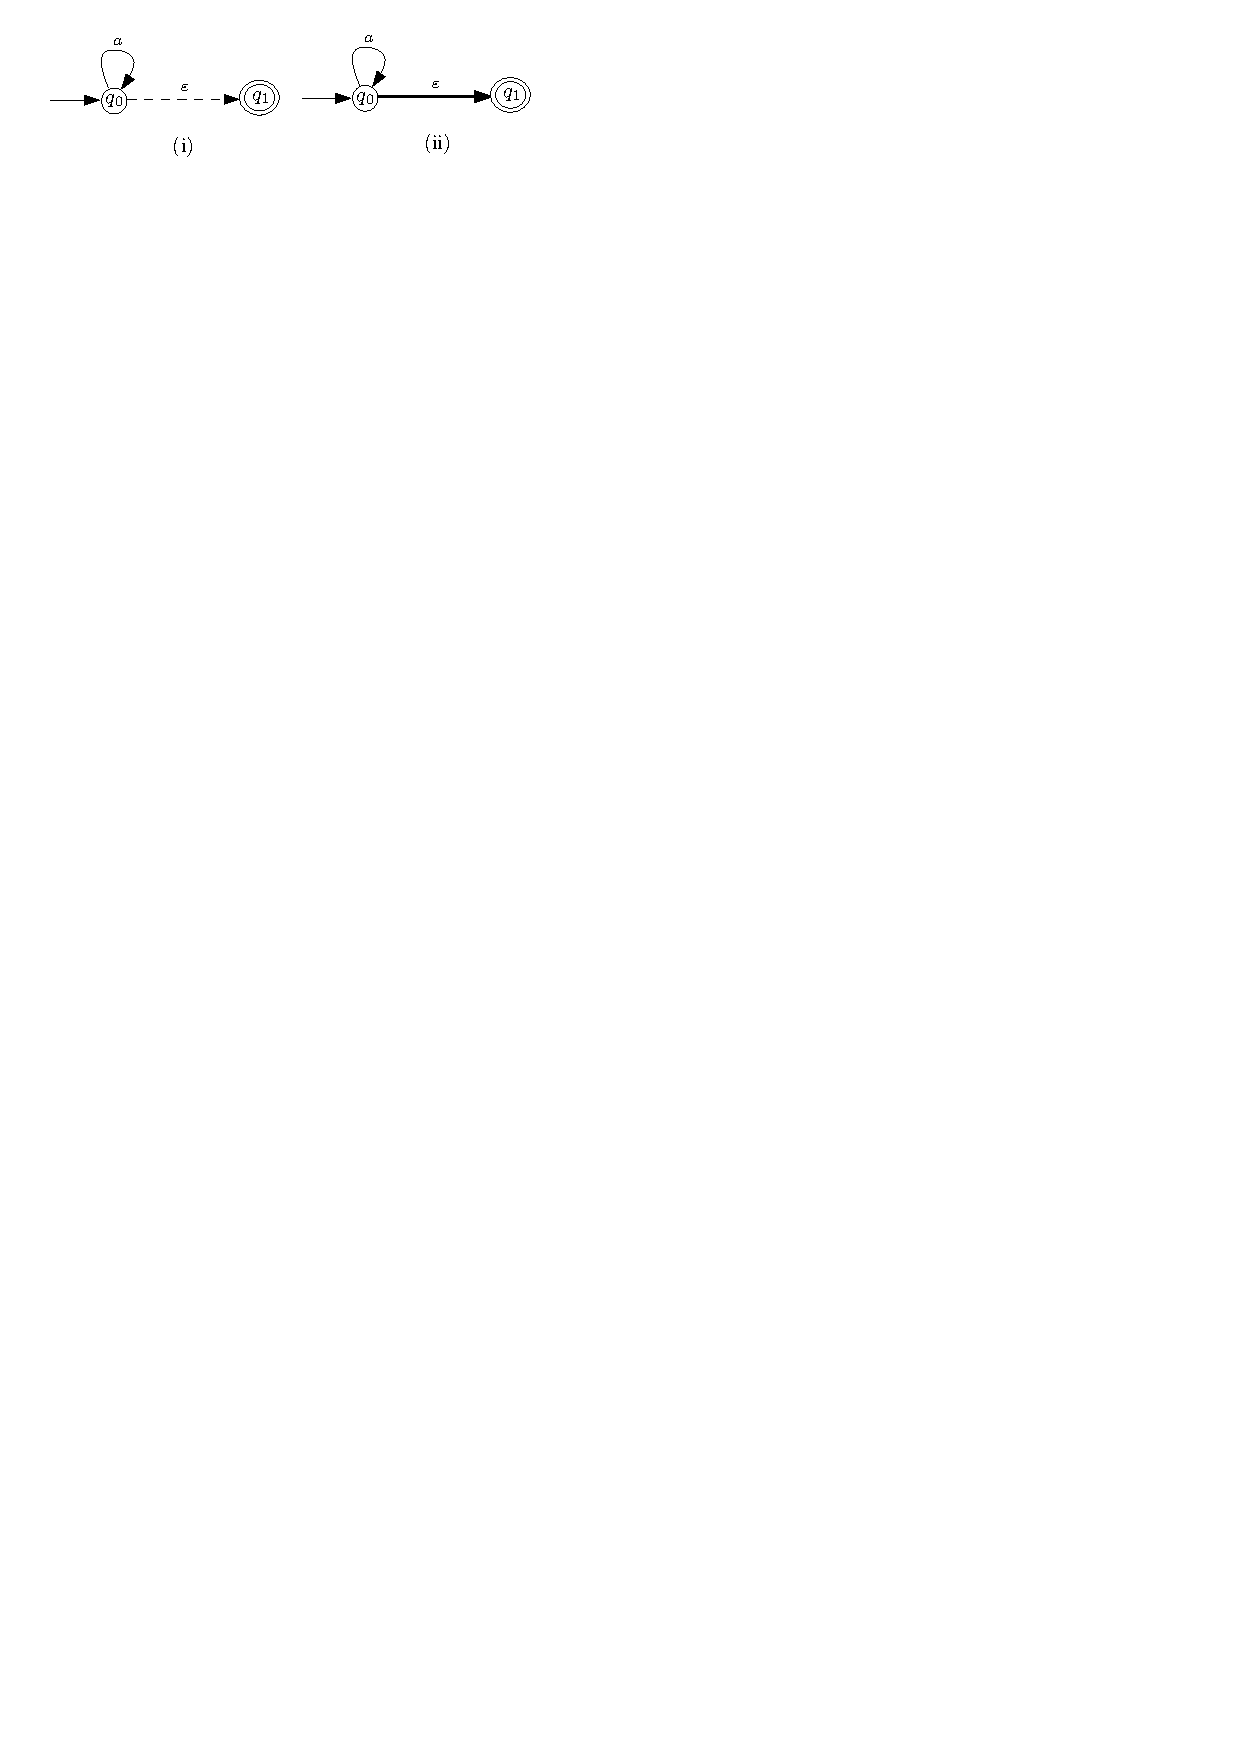
\includegraphics[width=0.6\textwidth]{pfa.pdf}
%\caption{The PFAs for $a^\ast$ and $a^{\ast?}$}
%\label{fig-pfa}
%\end{figure}
%\end{example}
%}
%%%%%%%%% The old example %%%%%%%%%

%\begin{remark}
%Remark that PFAs in Definition~\ref{def-pfa} are different from pNFAs in \cite{BM17} in the sense that the state set in a pNFA is partitioned into two disjoint subsets and the non-$\varepsilon$-transitions are deterministic, while this is not the case in PFAs. Therefore, PFAs are slightly more flexible than pNFAs in \cite{BM17}. We choose this definition of PFAs as a more natural extension of FAs. 
%\end{remark}

%The priorities of PFAs are used to model the greedy and non-greedy semantics of $\regexp$. %, as we shall see in Section~\ref{construction:pnfa}.
%
%\paragraph{Prioritized streaming string transducers.}
%

%%%%%%%%%%%%%%%%%%%%%%%%%%%%%%%%%%%%%%%%%%%%%%%%%%%%%%%%%%%%%%%%%%%%%%%%%%%%%%%%%%%%%%%%%%%%%%%%%%
%PSST
%%%%%%%%%%%%%%%%%%%%%%%%%%%%%%%%%%%%%%%%%%%%%%%%%%%%%%%%%%%%%%%%%%%%%%%%%%%%%%%%%%%%%%%%%%%%%%%%%%%%%%%
We are ready to define prioritized streaming string transducers. 
In the definition, the special symbol $\nullchar$ is introduced to capture the situation that $\extract_{i,e}(x)$ returns $\nullchar$, i.e. $x \in \Lang(e)$ but the $i$-th capturing group of $e$ is not matched.



%a new class of transducers that combine prioritized finite-state automata \cite{BM17} %which combines the expressive power of 
%and streaming string transducers \cite{AC10,AD11}.
  
  
\begin{definition}[Prioritized Streaming String Transducers]
A \emph{prioritized streaming string transducer} (PSST) is a tuple $\psst = (Q, \Sigma, X, \delta, \tau, E, q_0, F)$, where $Q$ is a
finite set of states, $\Sigma$ is the input and output alphabet such that $\nullchar \not \in \Sigma$, $X$ is a finite set of variables, $\delta \in Q \times \Sigma \rightarrow \overline{Q}$, $\tau \in Q \rightarrow \overline{Q} \times \overline{Q}$, $E$ is a partial function from $Q \times \Sigma^\varepsilon \times
  Q$ to $X \rightarrow \{\nullchar\} \cup (X \cup \Sigma)^{\ast}$, i.e. the set of assignments,
   $q_0 \in Q$ is the initial state, and $F$ is a partial function
  from $Q$ to $(X \cup \Sigma)^{\ast}$.
\end{definition}

A run of $\psst$ on a string $w$ is a sequence $q_0 a_1 s_1 q_1 \ldots a_m s_m q_m$ such that
\begin{itemize}
%\item $q_m \in F$,
%
\item for each $i \in [m]$, 
\begin{itemize}
\item either $a_i \in \Sigma$, $q_i \in \delta (q_{i-1}, a_i)$, and $s_i = E (q_{i - 1}, a_i, q_i)$, 
\item or $a_i = \varepsilon$, $q_i \in \tau(q_{i-1})$ and $s_i = E (q_{i - 1}, \varepsilon, q_i)$,
\end{itemize}

%\item for every subsequence $q_i a_{i+1} s_{i+1} q_{i+1} \ldots a_{j} s_j q_j$ such that  $i < j$ and $a_{i+1} = \cdots = a_j = \varepsilon$, it holds that $q_i, \ldots, q_j$ are mutually distinct. (Intuitively, loops of $\varepsilon$-transitions are forbidden.) 
\item for every subsequence $q_i a_{i+1} s_{i+1} q_{i+1} \ldots a_{j} s_j q_j$ such that  $i < j$ and $a_{i+1} = \cdots = a_j = \varepsilon$,  it holds that for every $k, l: i \le k < l < j$, $(q_k, q_{k+1}) \neq (q_l, q_{l+1})$.
\end{itemize}

%A run of $\psst$ is the sequence $q_0 a_1 s_1 q_1 \ldots a_m s_m q_m$, where $F (q_m)$ is defined and for each $i \in [m], q_i \in \delta (q_{i-1}, a_i)$ and $s_i = E (q_{i - 1}, a_i, q_i)$. 
For any pair of runs $R = q_0 a_1 s_1 \ldots a_m s_m q_m$ and $R' = q_0 a'_1
  s_1' \ldots a'_n s_n' q_n'$ such that $a_1 \ldots a_m = a'_1 \ldots a'_n$, the definition that $R$ is of a higher priority over
  $R'$ is similar to PFAs.
  % $p \neq p'$ and, for the smallest index $j$ with $q_j \neq q_j'$,
 % $\delta (q_{j - 1}, a_j) = \ldots q_j \ldots q_j' \ldots$
  
An accepting run of $\psst$ on $w$ is a run of $\psst$ on $w$, say $R = q_0 a_1 s_1 \ldots a_m s_m q_m$, such that 1) $F(q_m)$ is defined, 2)  $R$ is of the highest priority among those runs satisfying 1). The output of $\psst$ on $w$, denoted by $\psst(w)$, is defined as $\eta_m(F(q_m))$, where $\eta_0(x) = \varepsilon$ for each $x \in X$, and $\eta_{i}(x) = \eta_{i-1}(s_{i}(x))$ for every $1 \le i \le m$ and $x \in X$. Note that here we abuse the notation $\eta_m(F(q_m))$ and $\eta_{i-1}(s_{i}(x))$ by taking a function $\eta$ from $X$ to $(\Sigma \cup \{\nullchar\} )^*$ as a function from $(X \cup \Sigma \cup \{\nullchar\})^*$ to $(\Sigma \cup \{\nullchar\})^*$, which maps each $x \in X$ to $\eta(x)$, each $a \in \Sigma$ to $a$, and $\nullchar$ to $\nullchar$ . If there is no accepting run of $\psst$ on $w$, then $\psst(w) = \bot$, that is, the output of $\psst$ on $w$ is undefined. The string relation defined by $\psst$, denoted by $\cR_\psst$,  is 
$$\{(w, \psst(w)) \mid w \in \Sigma^\ast, \psst(w)  \in \Sigma^* \cup \{\nullchar\}\}.$$
Note that in the definition of $\cR_\psst$ above, the inputs of $\psst$ whose outputs are in $(\Sigma \cup \{\nullchar\})^* \setminus (\Sigma^* \cup \{\nullchar\})$ are ignored.


\begin{example}
The PSST $\cT_{\tt extract_{decimalReg,1}}=(Q, \Sigma, X, \delta, \tau, E,  q_{0}, F)$ mentioned in Section~\ref{sec:mot} is obtained from the PFA in Fig.~\ref{fig-pfa} by adding $x_1 := x_1 \ell$ to each $\ell$-transition going into $q_1$ (see Fig.~\ref{fig-psst-exmp}). More specifically, in $\cT_{\tt extract_{decimalReg,1}}$, we have $\Sigma = \{0,\cdots,9, .\}$, $X= \{x_1\}$ with $x_1$ recording the matches of the 1st capturing group, $F(q_{6}) = x_1$ denotes the final output, and $\delta, \tau, E$ are illustrated by the edges in Fig.~\ref{fig-psst-exmp}, where the dashed/ticker solid edges denote the $\varepsilon$-transitions of lower/higher priorities than the non-$\varepsilon$-transitions and the symbol $\ell$ is used to denote the currently scanned input letter. Note that the identity assignments, e.g. $E(q_3, ., q_4)(x_1) = x_1$, are omitted in Fig.~\ref{fig-psst-exmp}, for readability.   

%From $\delta(q_4, \backslash s) = q_5q_{6}$, we know that $q_5$ is prior to $q_6$. 
%Therefore, whenever $\cT_{\sf nameReg}$ reads $\backslash$s at the state $q_3$,  it will choose to go the state $q_5$ greedily, unless this choice would lead to the nonacceptance (in this case, $q_6$ will be chosen). 

\begin{figure*}[ht]

\centering
%\rule{\linewidth}{0cm}
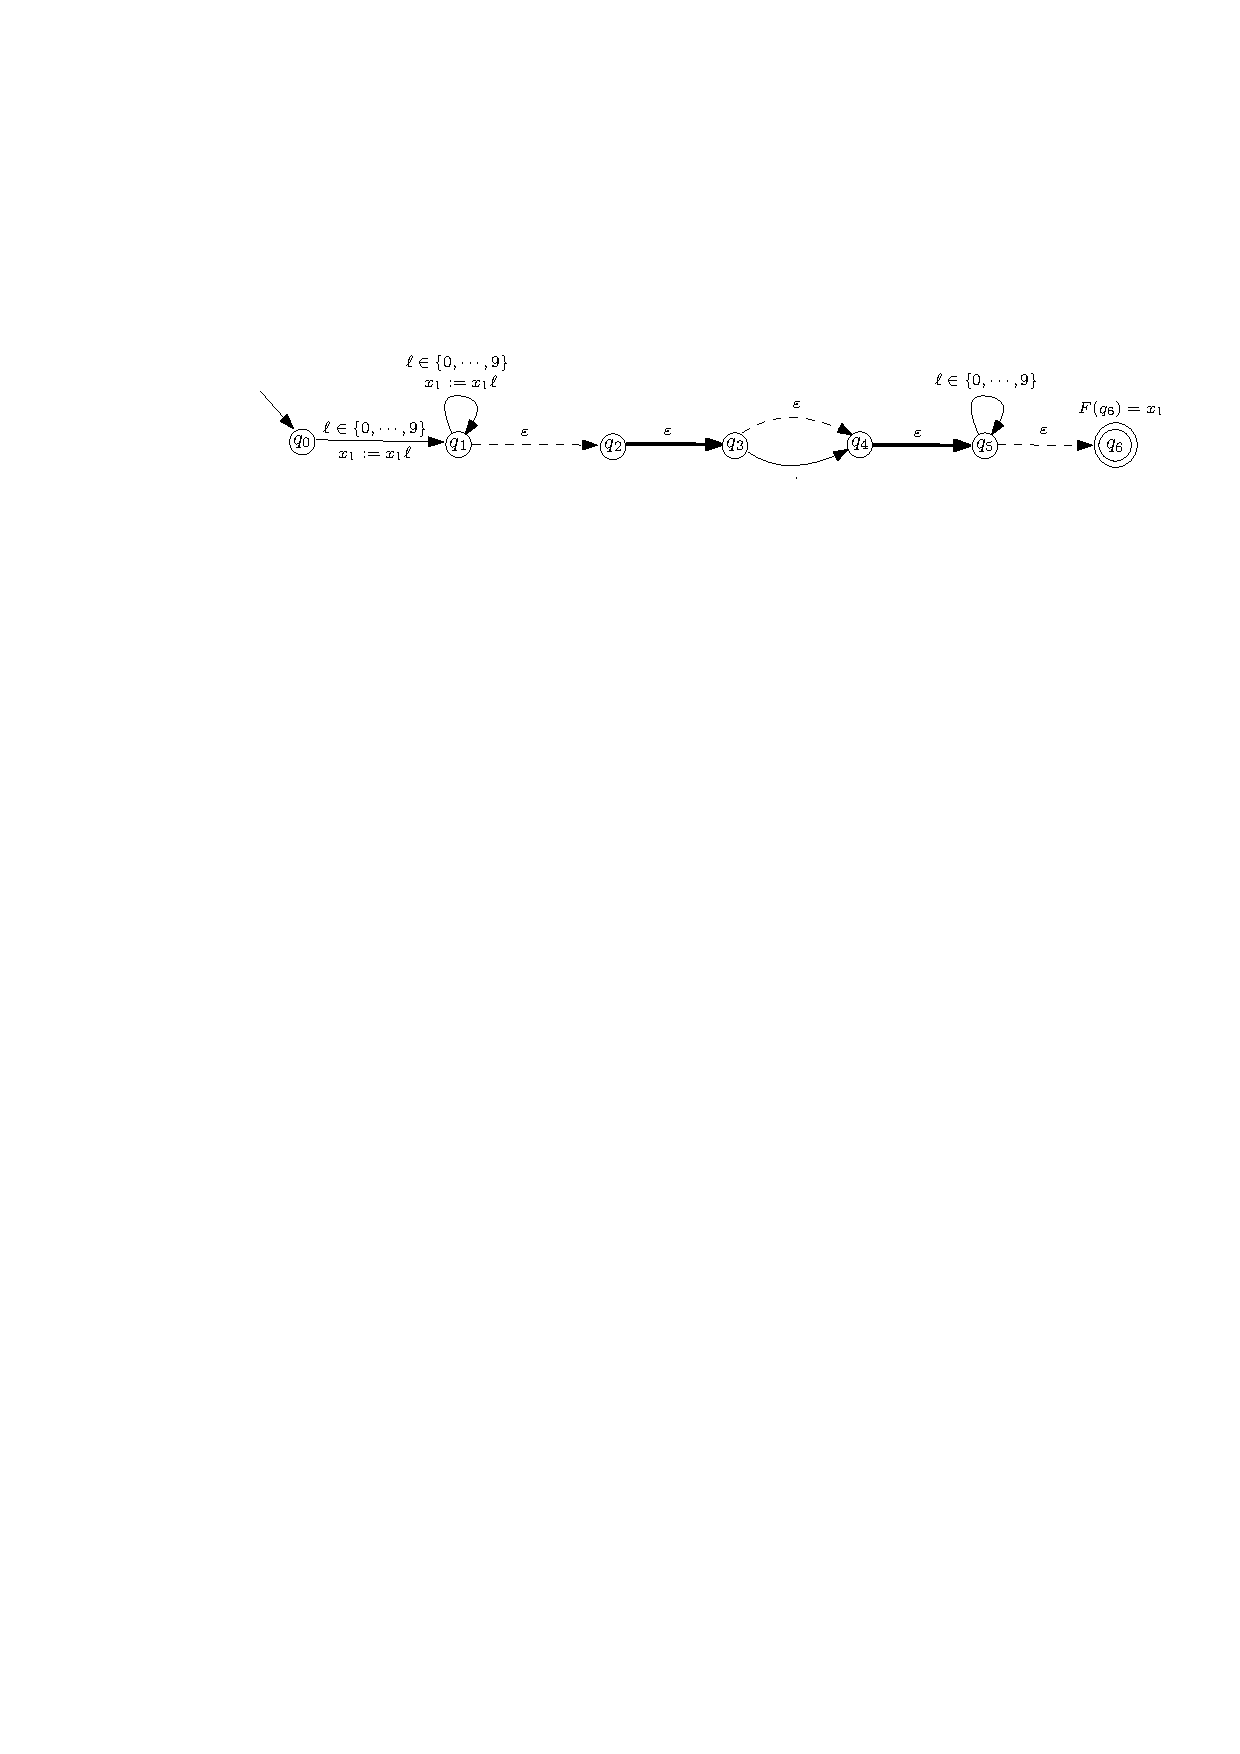
\includegraphics[width=0.95\textwidth]{psst-epsilon-exmp-new.pdf}
\caption{The PSST $\cT_{\tt extract_{decimalReg,1}}$}
\label{fig-psst-exmp}

\end{figure*}
\end{example}

  
%  $\tmop{Out} (r) =
%  s_{\varepsilon} \circ s_1 \circ s_2 \ldots s_n \circ F (q_n)$ where
%  $s_{\varepsilon}$ is the empty substitution which maps all variables to
%  $\varepsilon$.
  

% Note that in the definition of \NSST, there is no \emph{copyless} restriction.



